\documentclass[aspectratio=169,11pt]{beamer}

\usetheme{Madrid}
\usecolortheme{default}

\usepackage[utf8]{inputenc}
\usepackage[T1]{fontenc}
\usepackage[english]{babel}
\usepackage{graphicx}
\usepackage{booktabs}
\usepackage{tikz}
\usepackage{amsmath}
\usepackage{ragged2e}
\usepackage{adjustbox}

\graphicspath{{figures/}}
\usetikzlibrary{arrows.meta,positioning,shapes.geometric}

\definecolor{veripetblue}{RGB}{45,84,139}
\definecolor{veripetgreen}{RGB}{88,151,111}
\definecolor{veripetgray}{RGB}{72,76,82}
\definecolor{veripetlight}{RGB}{245,247,250}

\setbeamercolor{palette primary}{bg=veripetblue,fg=white}
\setbeamercolor{palette secondary}{bg=veripetgreen,fg=white}
\setbeamercolor{structure}{fg=veripetblue}
\setbeamercolor{frametitle}{bg=veripetblue,fg=white}
\setbeamercolor{block title}{bg=veripetblue,fg=white}
\setbeamercolor{block body}{bg=veripetlight,fg=black}
\setbeamercolor{alerted text}{fg=veripetgreen}
\setbeamertemplate{navigation symbols}{}
\setbeamertemplate{itemize item}{\color{veripetgreen}$\blacktriangleright$}
\setbeamertemplate{itemize subitem}{\color{veripetgreen}$\circ$}

\title[VeriPet]{VeriPet: Deep Learning-Based Dog Breed Classification and Individual Biometric Verification}
\subtitle{Research Article Presentation -- Artificial Intelligence}
\author{Raphael Damasceno Rocha de Moraes}
\institute[UNIFESP]{Graduate Program in Computer Science (PPG-CC)\\Universidade Federal de Sao Paulo -- UNIFESP}
\date{2026}

\newcommand{\metric}[2]{\textbf{\Large #1}\\{\footnotesize #2}}

\begin{document}

\begin{frame}
  \titlepage
  \vspace{-0.45cm}
  \begin{center}
    
\includegraphics[height=0.9cm]{logo-unifesp.pdf}
  \end{center}
\end{frame}

\begin{frame}{Presentation Roadmap}
  \begin{columns}[T,onlytextwidth]
    \begin{column}{0.48\textwidth}
      \begin{block}{Problem and Research Context}
        \begin{itemize}
          \item Motivation for canine biometrics
          \item Research gaps
          \item Related work and state of the art
          \item VeriPet research questions
        \end{itemize}
      \end{block}
    \end{column}
    \begin{column}{0.48\textwidth}
      \begin{block}{Experiments and Conclusions}
        \begin{itemize}
          \item Materials and methods
          \item Breed classification results
          \item Individual verification results
          \item Scientific impact and reproducibility
        \end{itemize}
      \end{block}
    \end{column}
  \end{columns}
\end{frame}

\begin{frame}{Motivation}
  \begin{columns}[T,onlytextwidth]
    \begin{column}{0.57\textwidth}
      \begin{itemize}
        \item Dog identification supports lost-pet recovery, shelter management, animal welfare, and responsible ownership policies.
        \item Traditional identifiers have operational limits: collars can be lost and microchips require physical access and dedicated readers.
        \item Camera-based identification can be non-invasive, low-cost, and scalable.
        \item The AI challenge is robust recognition under pose, illumination, framing, resolution, age, fur, and occlusion variation.
      \end{itemize}
    \end{column}
    \begin{column}{0.39\textwidth}
      \begin{alertblock}{Central Idea}
        Learn visual representations that support dog breed recognition and individual biometric verification.
      \end{alertblock}
      \begin{block}{Research Focus}
        Evaluate modern deep learning models and the role of breed information in identity verification.
      \end{block}
    \end{column}
  \end{columns}
\end{frame}

\begin{frame}{Computational Challenge}
  \begin{columns}[T,onlytextwidth]
    \begin{column}{0.48\textwidth}
      \begin{block}{Intra-class Variation}
        The same dog may appear with different:
        \begin{itemize}
          \item poses and camera angles;
          \item lighting and image quality;
          \item age, fur state, and occlusions.
        \end{itemize}
      \end{block}
    \end{column}
    \begin{column}{0.48\textwidth}
      \begin{block}{Inter-class Similarity}
        Different dogs can look very similar, especially:
        \begin{itemize}
          \item within the same breed;
          \item across related breeds;
          \item in close facial crops.
        \end{itemize}
      \end{block}
    \end{column}
  \end{columns}

  \vspace{0.25cm}
  \begin{center}
    \begin{minipage}{0.72\textwidth}
      \begin{alertblock}{Key Evaluation Need}
        Verification must report intra-breed performance, not only global accuracy.
      \end{alertblock}
    \end{minipage}
  \end{center}
\end{frame}

\begin{frame}{Research Gaps}
  \begin{columns}[T,onlytextwidth]
    \begin{column}{0.50\textwidth}
      \begin{block}{Known Progress}
        \begin{itemize}
          \item Animal biometrics can exploit natural visual patterns.
          \item Deep models improved fine-grained dog breed classification.
          \item PetFace enables larger-scale animal identity evaluation.
        \end{itemize}
      \end{block}
    \end{column}
    \begin{column}{0.46\textwidth}
      \begin{alertblock}{Open Problems}
        \begin{itemize}
          \item Few standardized public protocols for canine biometrics.
          \item Breed labels do not directly solve identity verification.
          \item Limited analysis of breed as a complementary verification signal.
        \end{itemize}
      \end{alertblock}
    \end{column}
  \end{columns}
\end{frame}

\begin{frame}{State of the Art Used in VeriPet}
  \begin{columns}[T,onlytextwidth]
    \begin{column}{0.48\textwidth}
      \begin{block}{Image Recognition}
        \begin{itemize}
          \item Transfer learning from ImageNet.
          \item ConvNeXt as a modern convolutional backbone.
          \item Fine-grained recognition over 120 dog breeds.
        \end{itemize}
      \end{block}
    \end{column}
    \begin{column}{0.48\textwidth}
      \begin{block}{Identity Verification}
        \begin{itemize}
          \item Embedding-based comparison.
          \item Cosine similarity for pair decisions.
          \item ArcFace angular-margin loss for stronger separation.
        \end{itemize}
      \end{block}
    \end{column}
  \end{columns}

  \vspace{0.25cm}
  \begin{alertblock}{Limitation}
    Generic classification accuracy is not enough: biometric identity requires a discriminative embedding space.
  \end{alertblock}
\end{frame}

\begin{frame}{Research Questions}
  \begin{block}{Main Question}
    Can deep learning support reliable individual dog verification from images while using breed information as complementary context?
  \end{block}

  \begin{columns}[T,onlytextwidth]
    \begin{column}{0.48\textwidth}
      \begin{itemize}
        \item How well does ConvNeXt classify 120 dog breeds?
        \item How effective are ConvNeXt embeddings for individual verification?
      \end{itemize}
    \end{column}
    \begin{column}{0.48\textwidth}
      \begin{itemize}
        \item Does ArcFace improve canine identity embeddings?
        \item Can breed compatibility improve or explain verification decisions?
      \end{itemize}
    \end{column}
  \end{columns}
\end{frame}

\begin{frame}{Conceptual VeriPet Pipeline}
  \centering
  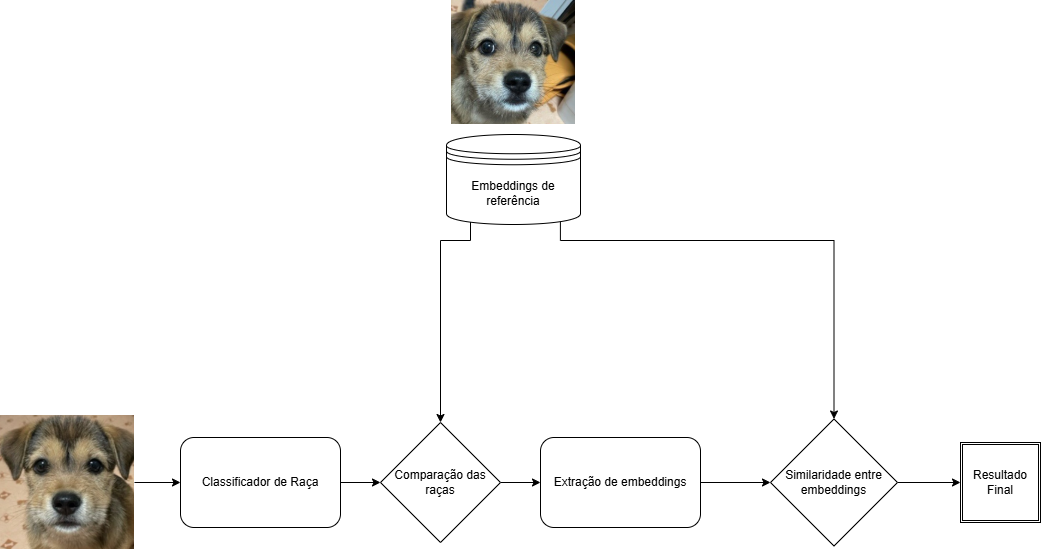
\includegraphics[width=0.98\textwidth,height=0.72\textheight,keepaspectratio]{pipeline_veripet.png}
\end{frame}

\begin{frame}{Final Experimental Scope}
  \centering
  \resizebox{0.96\textwidth}{!}{%
  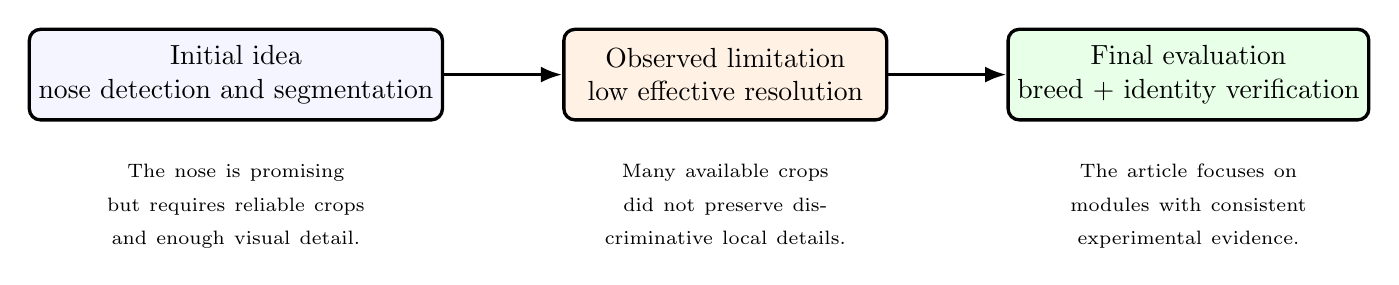
\begin{tikzpicture}[
    node distance=1.5cm,
    box/.style={draw, rounded corners, very thick, align=center, minimum width=4.0cm, minimum height=1.15cm, fill=blue!4},
    warn/.style={draw, rounded corners, very thick, align=center, minimum width=4.1cm, minimum height=1.15cm, fill=orange!10},
    keep/.style={draw, rounded corners, very thick, align=center, minimum width=4.2cm, minimum height=1.15cm, fill=green!9},
    arrow/.style={-{Latex[length=2.7mm]}, very thick}
  ]
    \node[box] (idea) {Initial idea\\nose detection and segmentation};
    \node[warn, right=of idea] (limit) {Observed limitation\\low effective resolution};
    \node[keep, right=of limit] (scope) {Final evaluation\\breed + identity verification};

    \draw[arrow] (idea) -- (limit);
    \draw[arrow] (limit) -- (scope);

    \node[below=0.42cm of idea, align=center, text width=3.8cm] {\scriptsize The nose is promising but requires reliable crops and enough visual detail.};
    \node[below=0.42cm of limit, align=center, text width=4.0cm] {\scriptsize Many available crops did not preserve discriminative local details.};
    \node[below=0.42cm of scope, align=center, text width=4.0cm] {\scriptsize The article focuses on modules with consistent experimental evidence.};
  \end{tikzpicture}}

  \vspace{0.25cm}
  \begin{block}{Methodological Decision}
    Nose segmentation was considered but not included in the final evaluation to preserve experimental validity.
  \end{block}
\end{frame}

\begin{frame}{Materials: Datasets}
  \begin{columns}[T,onlytextwidth]
    \begin{column}{0.48\textwidth}
      \begin{block}{Breed Classification: Stanford Dogs}
        \begin{itemize}
          \item 20,580 images.
          \item 120 dog breeds.
          \item Bounding-box annotations.
          \item Stratified split: 70\% train, 15\% validation, 15\% test.
        \end{itemize}
      \end{block}
    \end{column}
    \begin{column}{0.48\textwidth}
      \begin{block}{Verification: PetFace Dog}
        \begin{itemize}
          \item 46,755 identities.
          \item 168,348 training images.
          \item 35,366 balanced test pairs.
          \item Same-breed pairs used for intra-breed evaluation.
        \end{itemize}
      \end{block}
    \end{column}
  \end{columns}
\end{frame}

\begin{frame}{PetFace Dog: Exploratory Analysis}
  \begin{columns}[T,onlytextwidth]
    \begin{column}{0.40\textwidth}
      \centering
      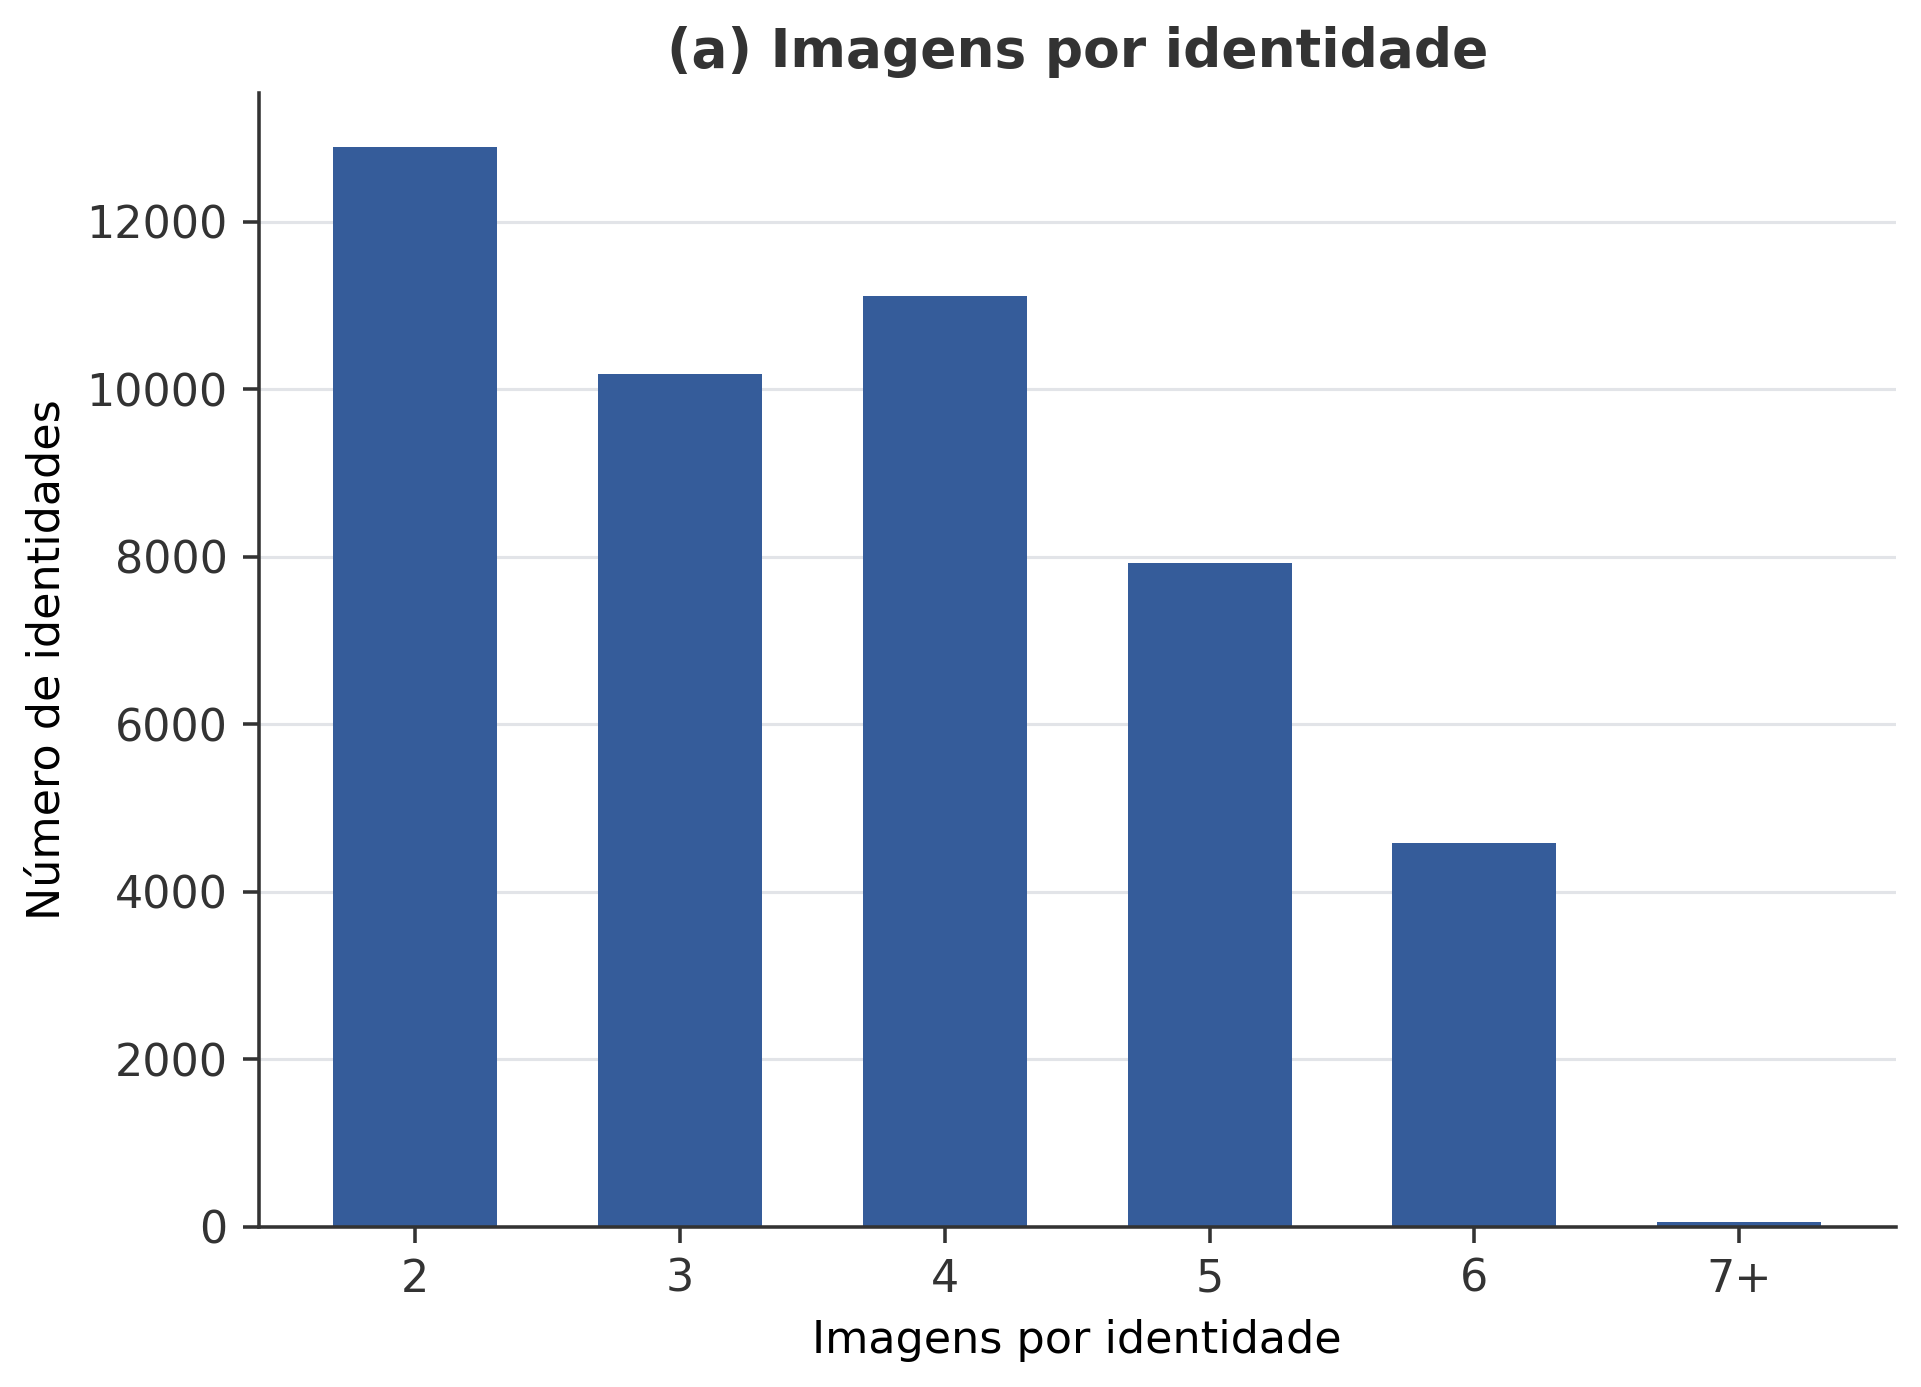
\includegraphics[width=\textwidth,height=0.62\textheight,keepaspectratio]{eda_distributions_a.png}
    \end{column}
    \begin{column}{0.57\textwidth}
      \centering
      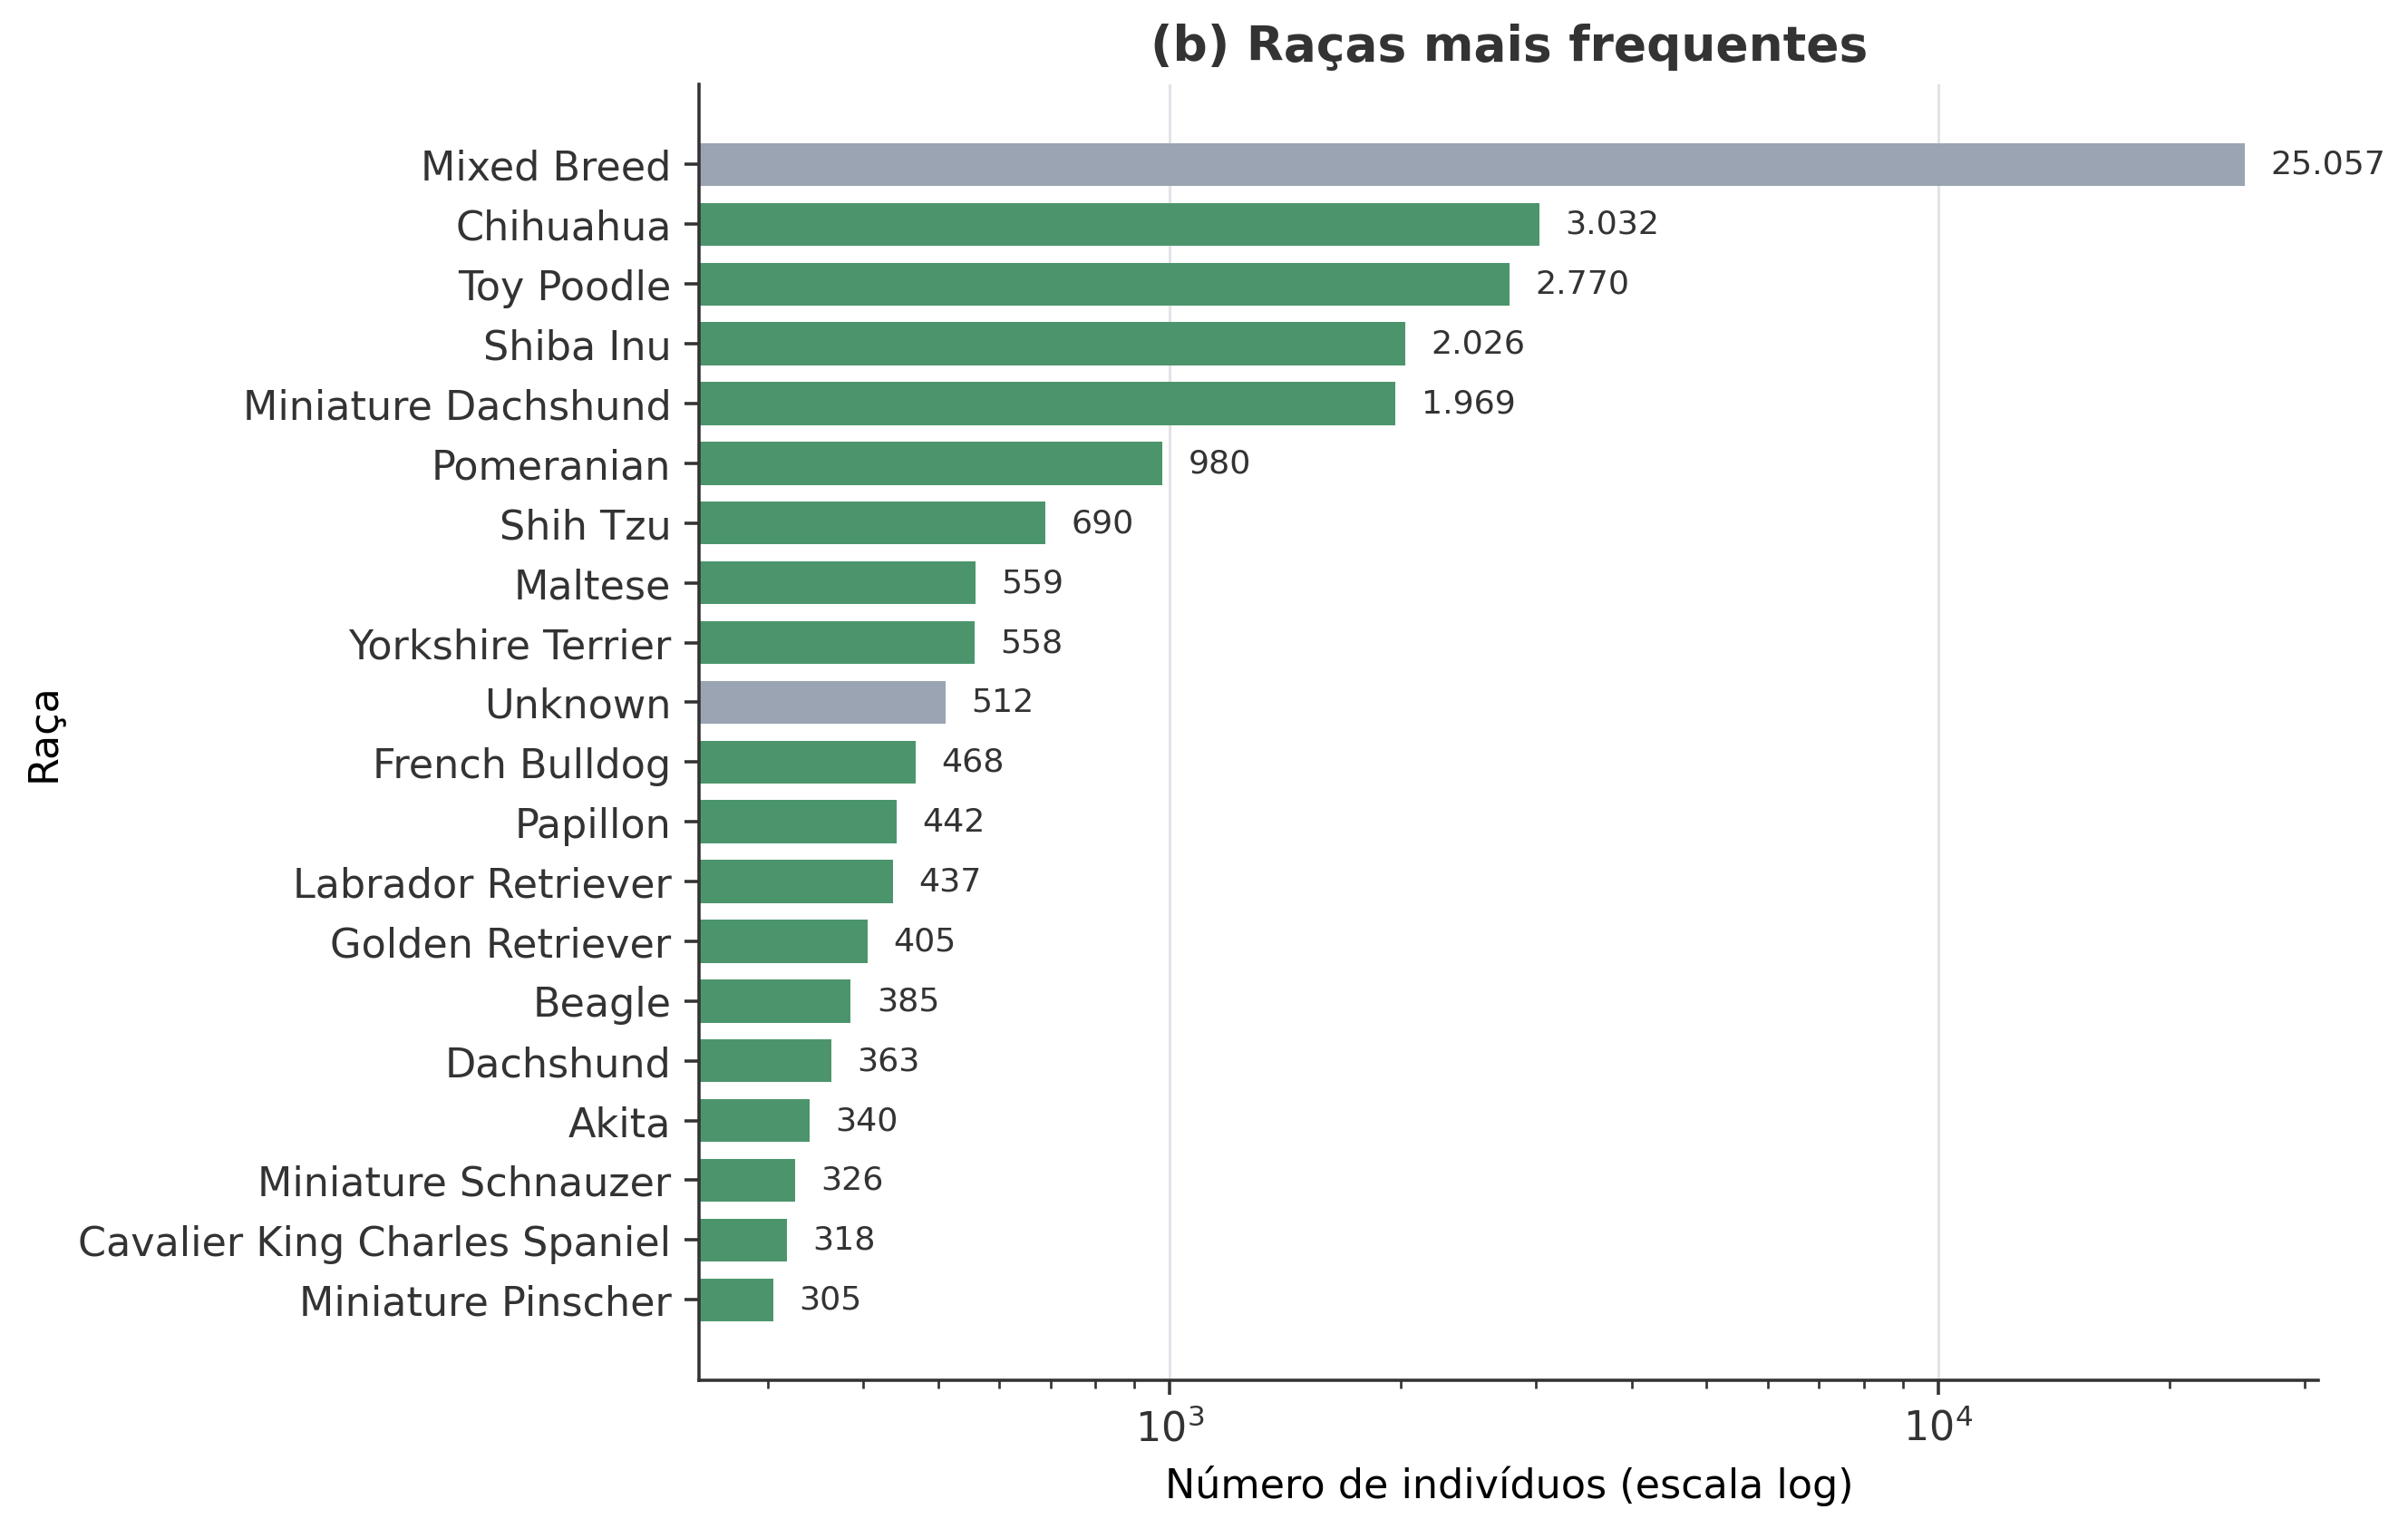
\includegraphics[width=\textwidth,height=0.62\textheight,keepaspectratio]{eda_distributions_b.png}
    \end{column}
  \end{columns}
\end{frame}

\begin{frame}{Methodology Summary}
  \begin{columns}[T,onlytextwidth]
    \begin{column}{0.48\textwidth}
      \begin{table}
        \centering
        \caption{Breed Classifier}
        \small
        \begin{tabular}{ll}
          \toprule
          Item & Value \\
          \midrule
          Backbone & ConvNeXt-Tiny \\
          Pretraining & ImageNet-1K \\
          Loss & Cross-Entropy \\
          Batch size & 256 \\
          Optimizer & AdamW \\
          Selection & Validation loss \\
          \bottomrule
        \end{tabular}
      \end{table}
    \end{column}
    \begin{column}{0.48\textwidth}
      \begin{table}
        \centering
        \caption{Identity Verifier}
        \small
        \begin{tabular}{ll}
          \toprule
          Item & Value \\
          \midrule
          Backbone & ConvNeXt-Small \\
          Embedding & 768 dimensions \\
          Losses & Softmax, ArcFace \\
          Batch size & 128 \\
          Optimizer & AdamW \\
          Selection & Validation AUC \\
          \bottomrule
        \end{tabular}
      \end{table}
    \end{column}
  \end{columns}
\end{frame}

\begin{frame}{Breed Classification: Results}
  \begin{columns}[T,onlytextwidth]
    \begin{column}{0.43\textwidth}
      \begin{table}
        \centering
        \small
        \begin{tabular}{lr}
          \toprule
          Metric & Value \\
          \midrule
          Global accuracy & 92.55\% \\
          Macro precision & 92.8\% \\
          Macro recall & 92.5\% \\
          Macro-F1 & 92.4\% \\
          Weighted-F1 & 92.6\% \\
          \bottomrule
        \end{tabular}
      \end{table}
      \begin{block}{Interpretation}
        \small Results were measured on the held-out Stanford Dogs test set with 3,087 images. The model generalizes well across 120 breeds.
      \end{block}
    \end{column}
    \begin{column}{0.54\textwidth}
      \centering
      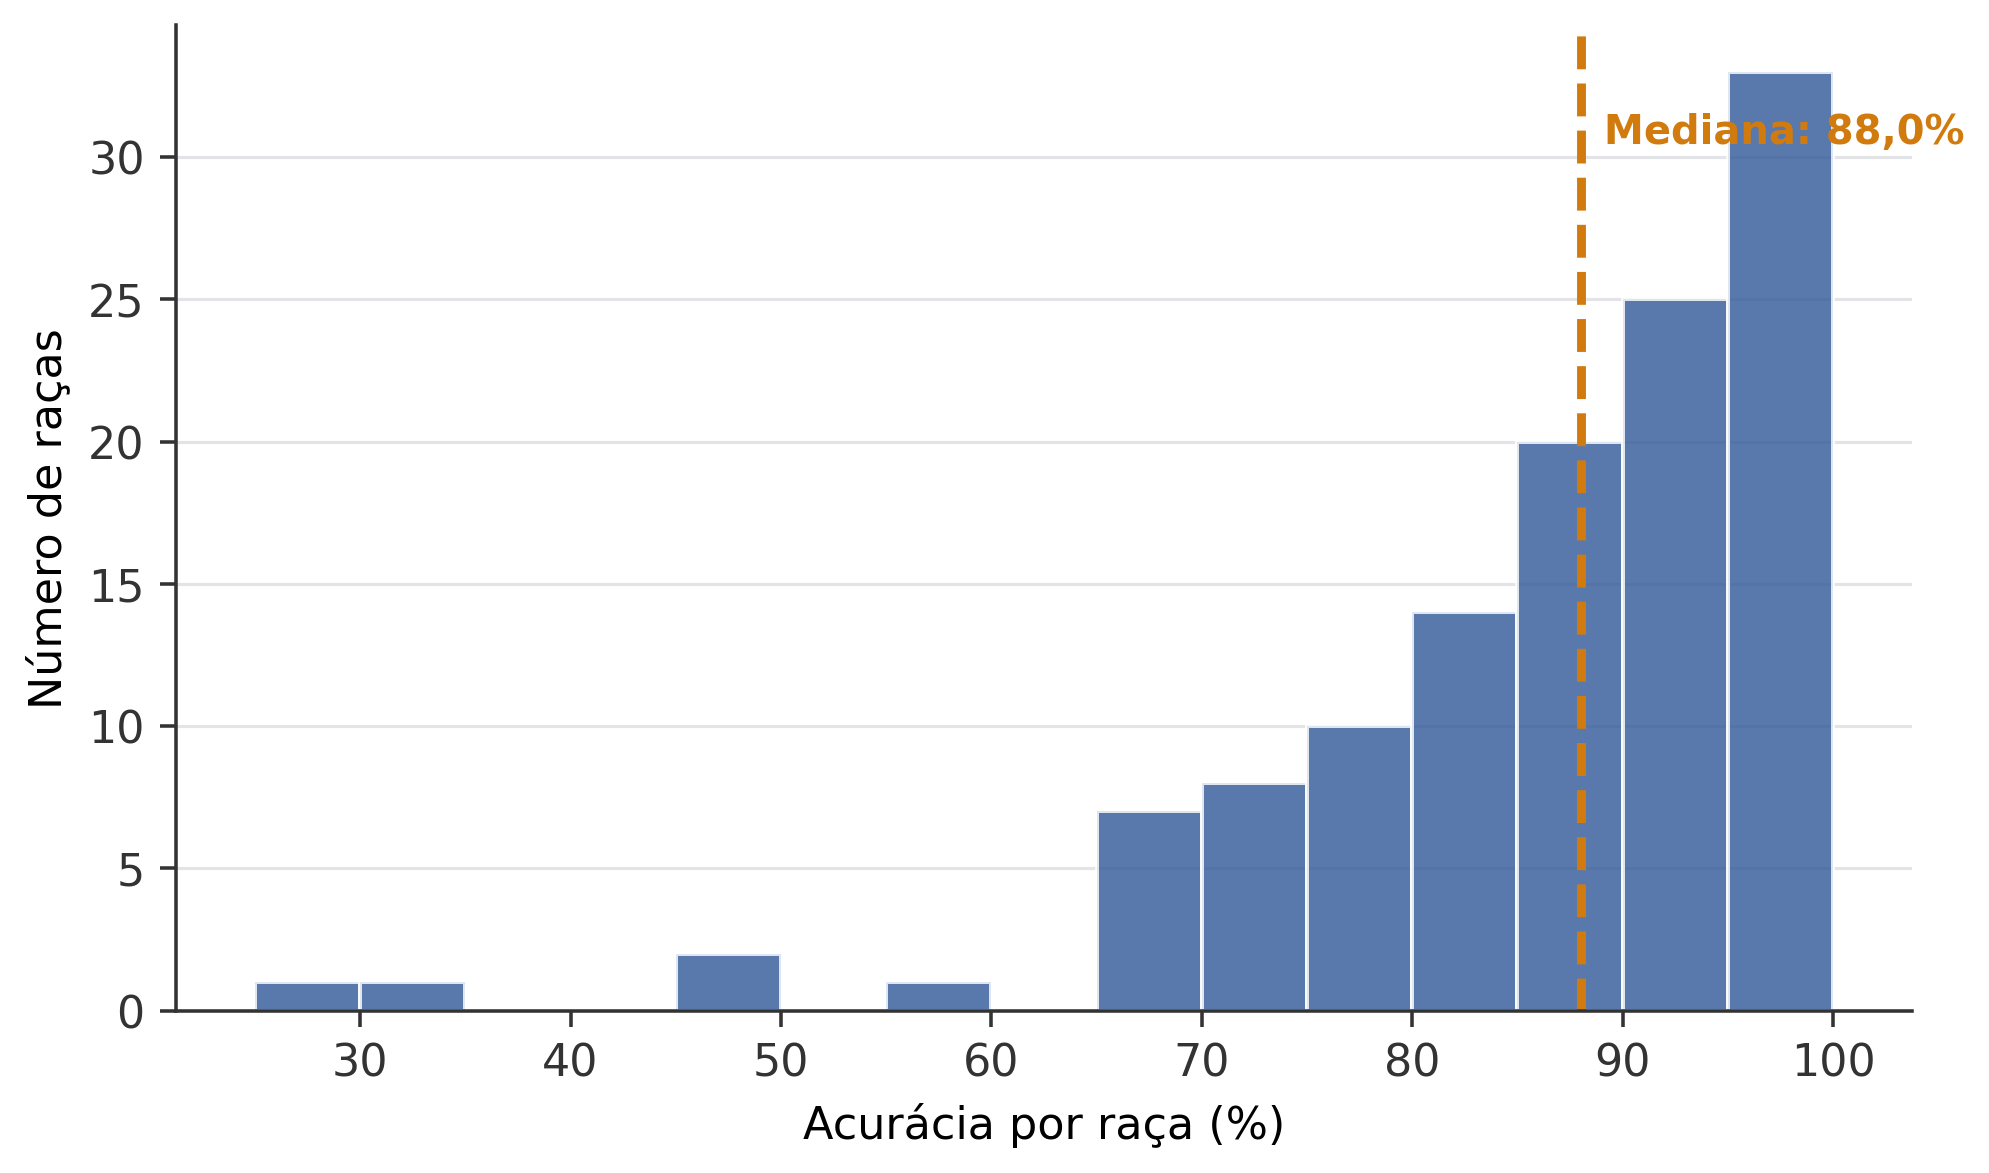
\includegraphics[width=\textwidth,height=0.56\textheight,keepaspectratio]{distribuicao_acuracias.png}
    \end{column}
  \end{columns}
\end{frame}

\begin{frame}{Breed Classification: Qualitative Examples}
  \centering
  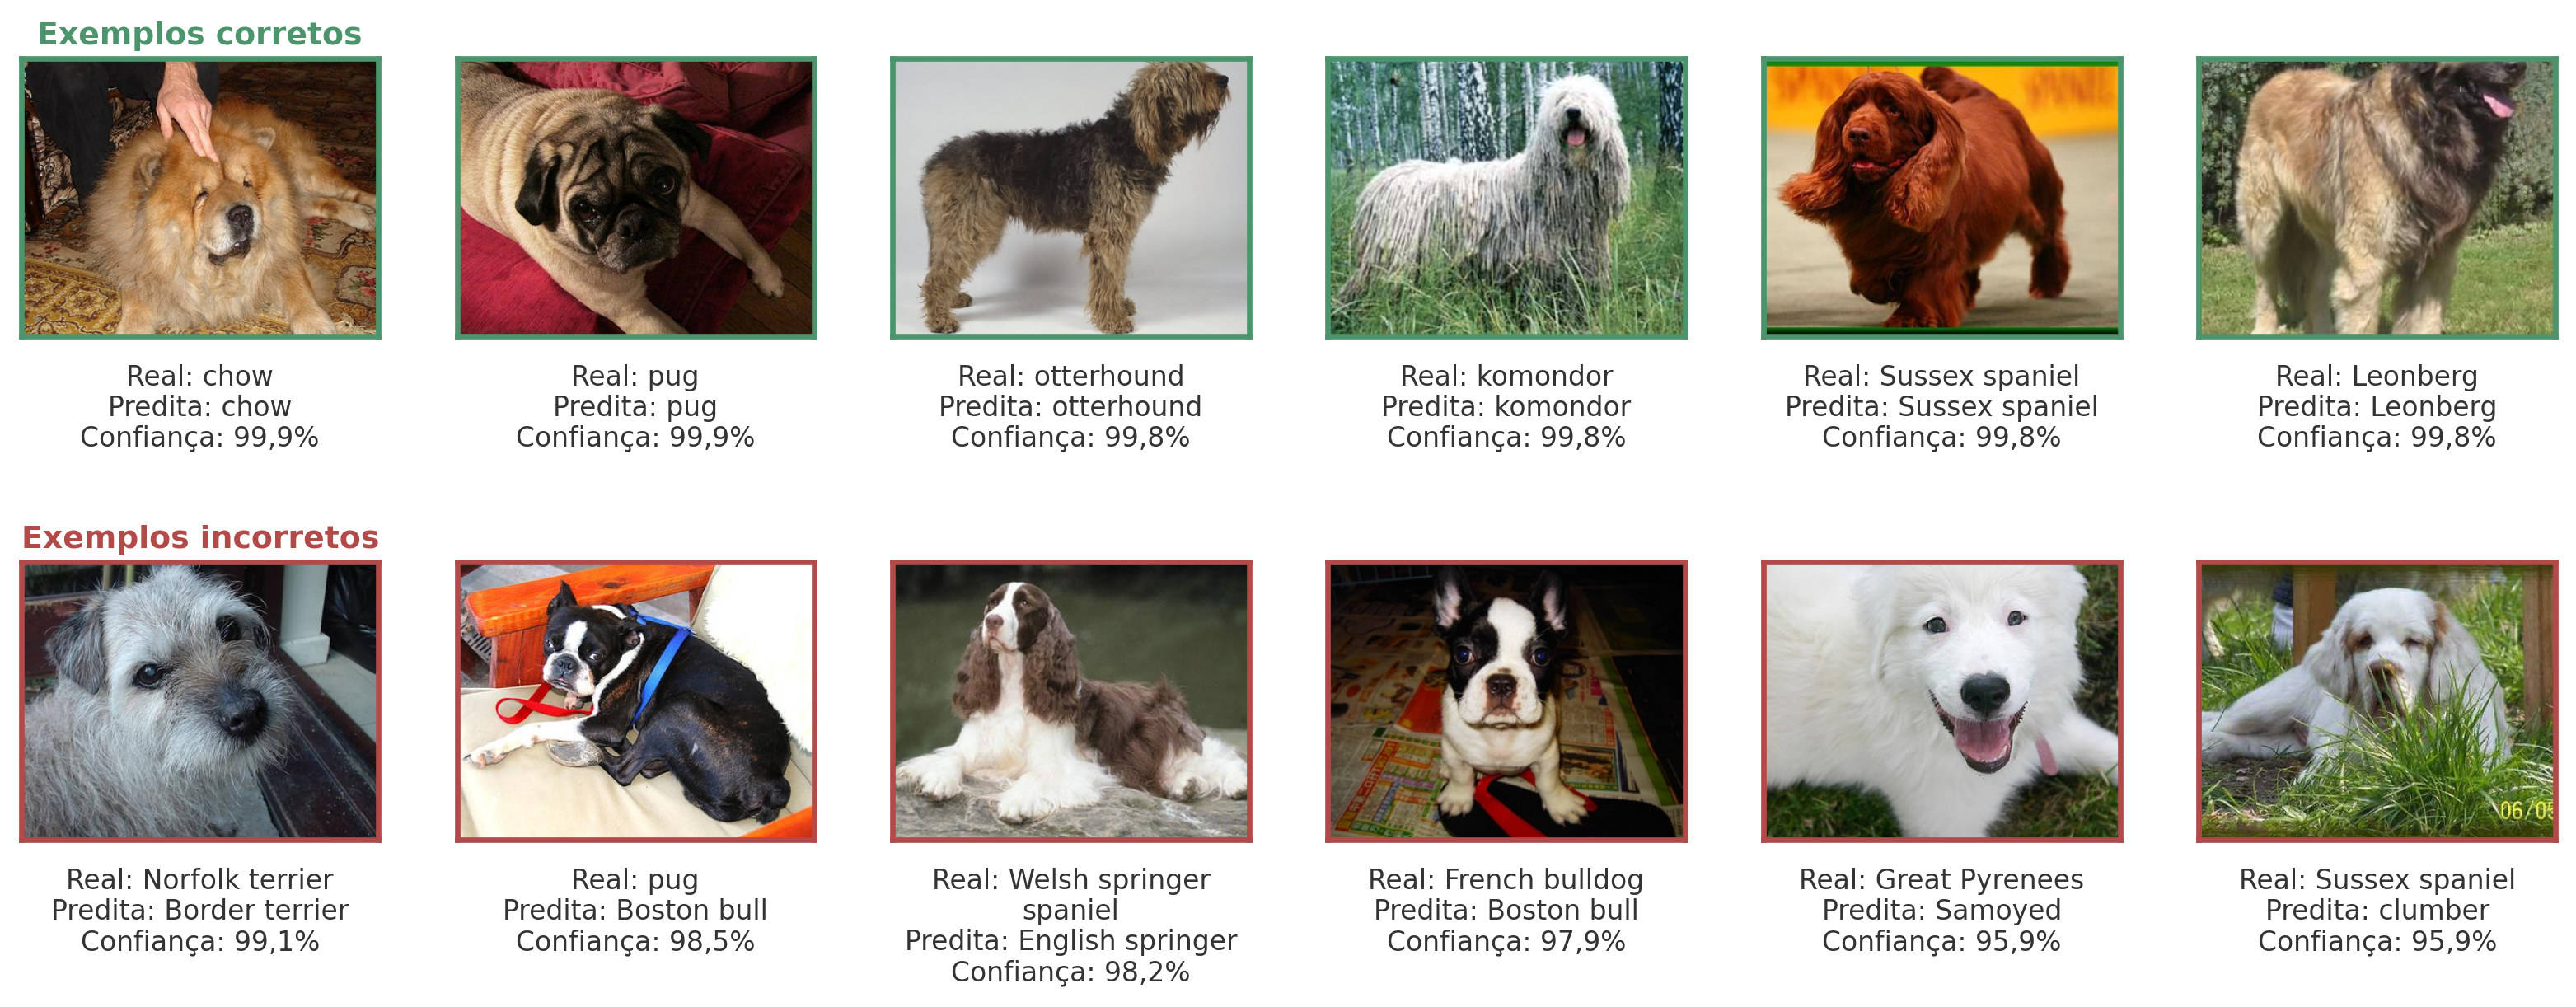
\includegraphics[width=0.96\textwidth,height=0.68\textheight,keepaspectratio]{amostras_predicoes.png}
\end{frame}

\begin{frame}{Breed Error Analysis}
  \begin{table}
    \centering
    \scriptsize
    \begin{tabular}{lrrl}
      \toprule
      True breed & Errors & Accuracy & Main confusion \\
      \midrule
      wire-haired fox terrier & 8 & 66.7\% & Lakeland terrier \\
      Border collie & 7 & 68.2\% & collie \\
      Eskimo dog & 6 & 72.7\% & Siberian husky \\
      Staffordshire bullterrier & 6 & 73.9\% & Am. Staffordshire terrier \\
      miniature poodle & 6 & 73.9\% & toy poodle \\
      standard schnauzer & 6 & 73.9\% & miniature schnauzer \\
      \bottomrule
    \end{tabular}
  \end{table}
  \begin{columns}[T,onlytextwidth]
    \begin{column}{0.32\textwidth}
      \begin{block}{Visual Pairs}
        Husky/Eskimo, Border collie/collie.
      \end{block}
    \end{column}
    \begin{column}{0.32\textwidth}
      \begin{block}{Scale Variants}
        Poodles and schnauzers in different sizes.
      \end{block}
    \end{column}
    \begin{column}{0.32\textwidth}
      \begin{block}{Functional Groups}
        Terriers and genetically related breeds.
      \end{block}
    \end{column}
  \end{columns}
\end{frame}

\begin{frame}{Misclassification Mosaics}
  \centering
  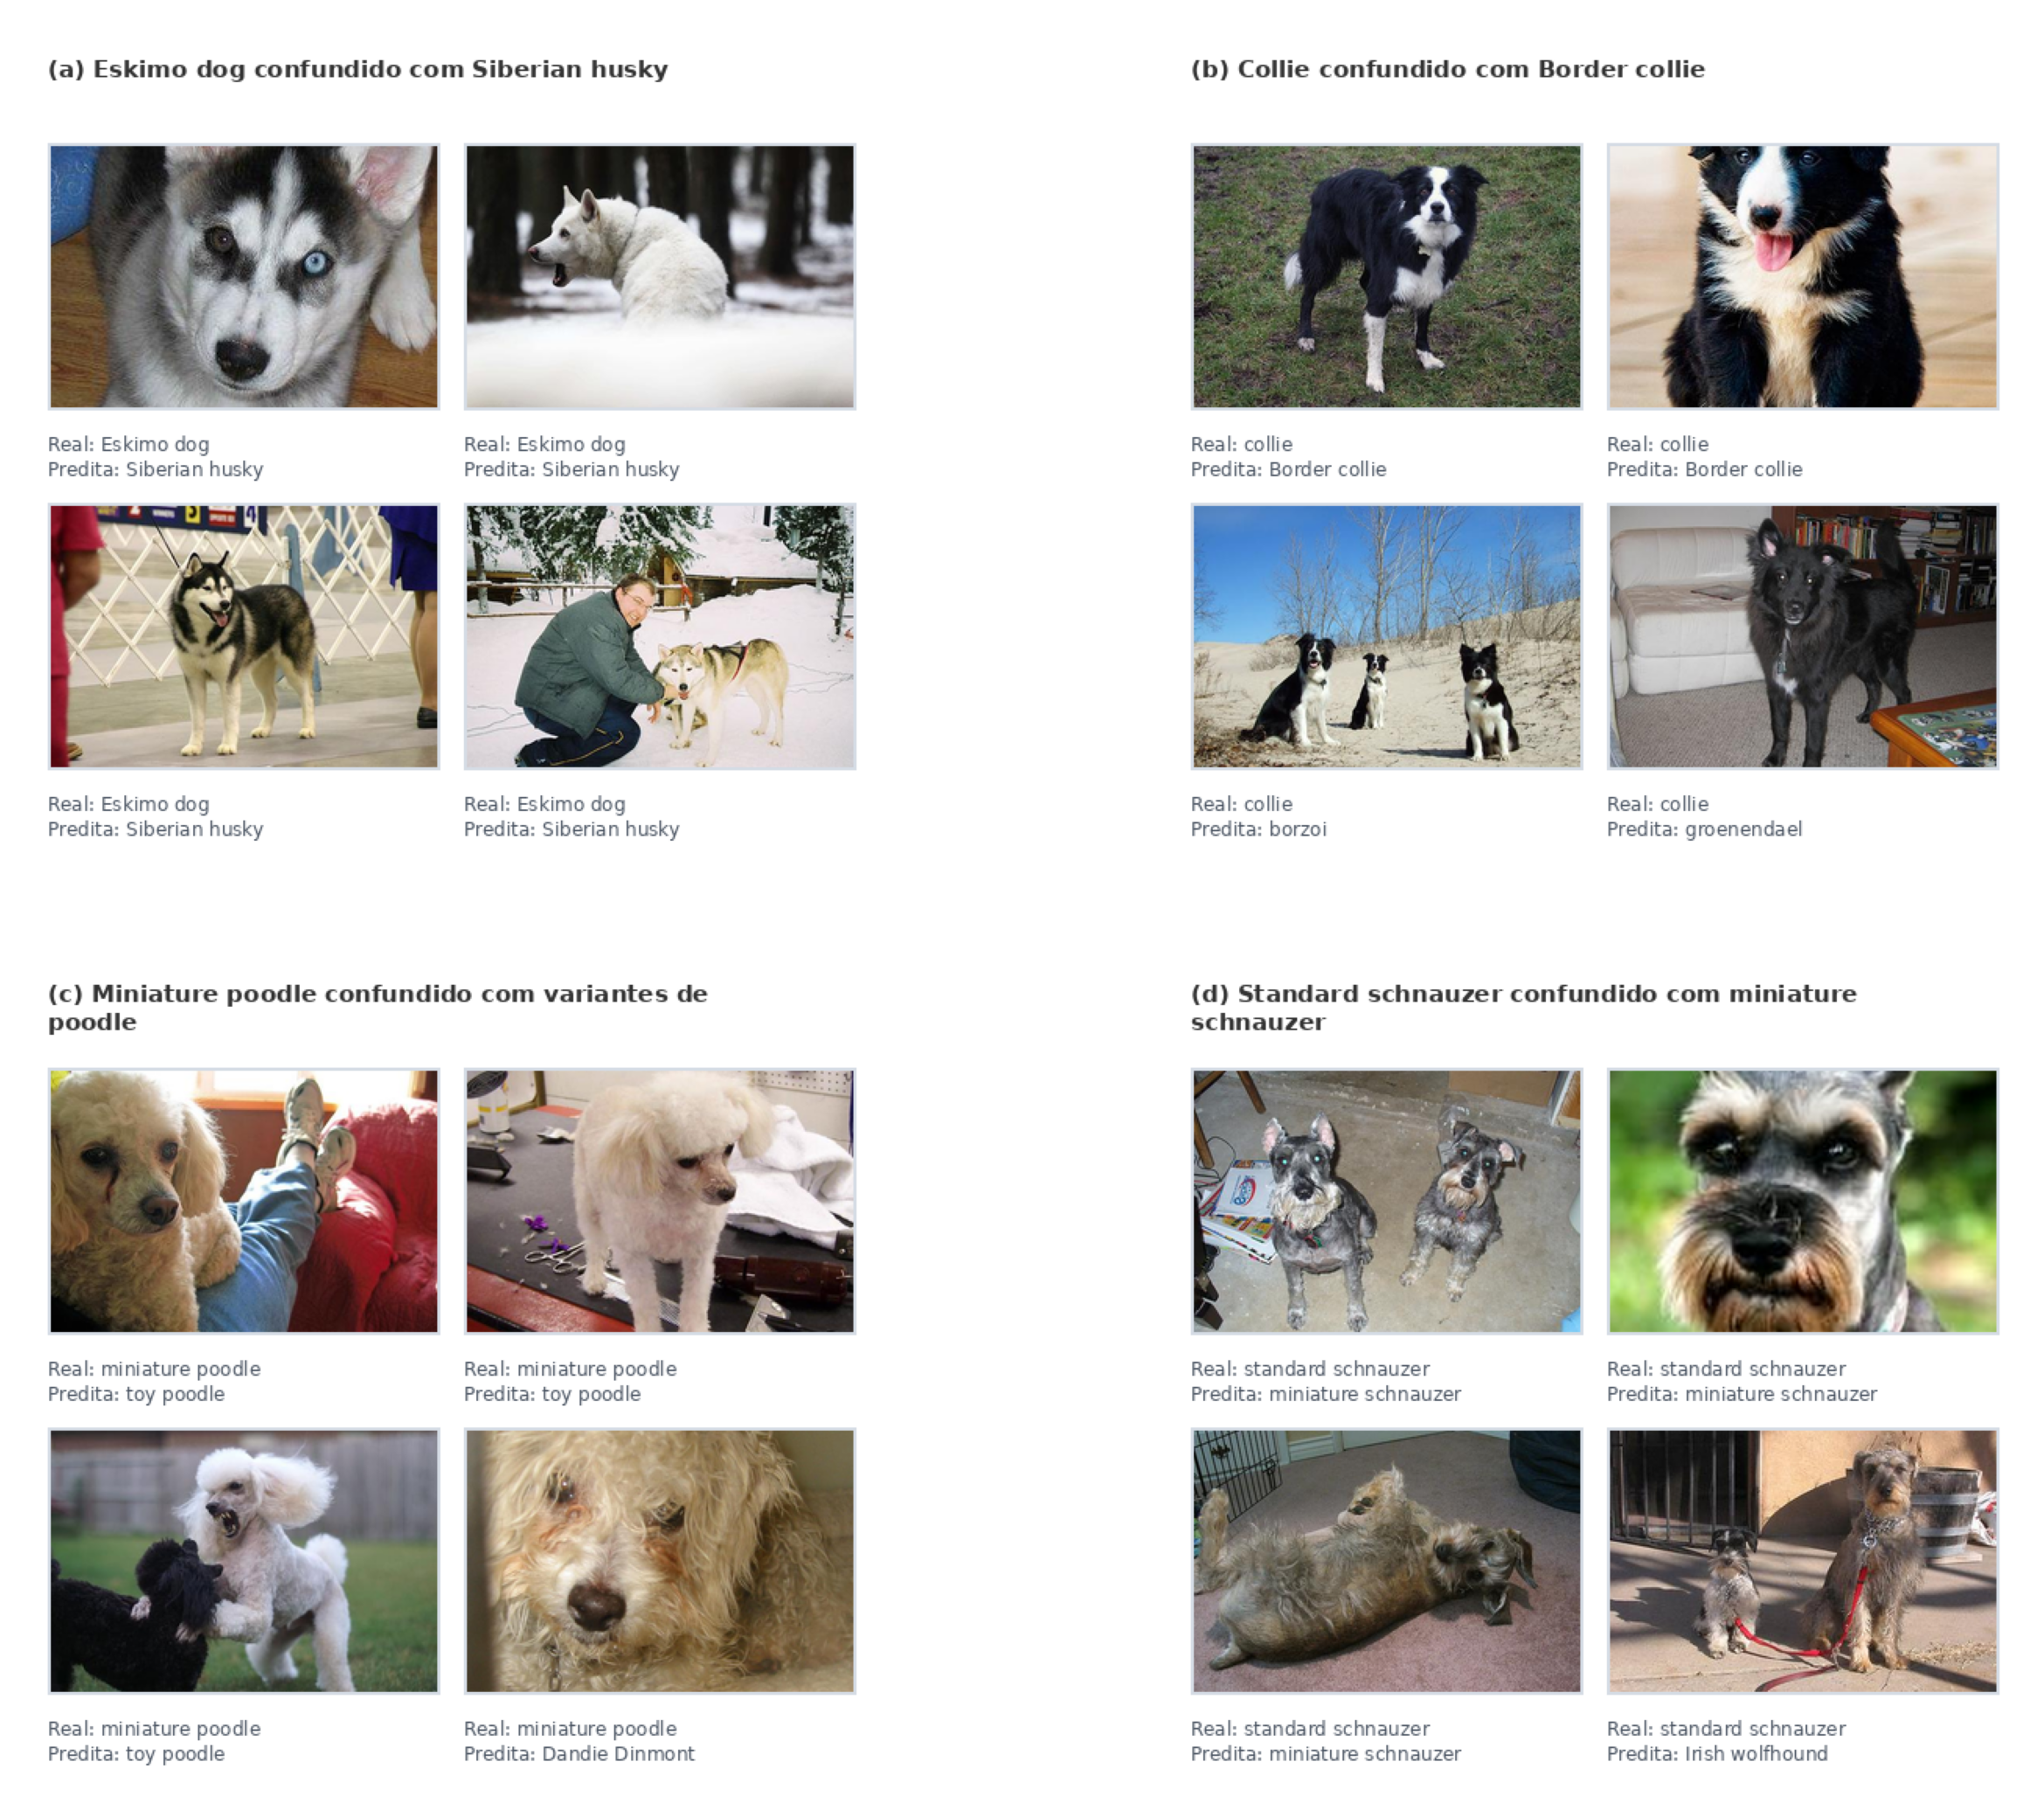
\includegraphics[width=0.98\textwidth,height=0.70\textheight,keepaspectratio]{mosaicos_erros_2x2.png}
\end{frame}

\begin{frame}{Individual Verification: Method}
  \begin{columns}[T,onlytextwidth]
    \begin{column}{0.50\textwidth}
      \begin{block}{Input}
        A pair of images: same dog or different dogs.
      \end{block}
      \begin{block}{Representation}
        ConvNeXt-Small produces 768-dimensional embeddings.
      \end{block}
    \end{column}
    \begin{column}{0.46\textwidth}
      \begin{block}{Decision}
        Cosine similarity is compared with a validation-calibrated threshold.
      \end{block}
      \begin{alertblock}{Critical Scenario}
        Intra-breed accuracy measures pairs where both dogs belong to the same breed.
      \end{alertblock}
    \end{column}
  \end{columns}
  \vspace{0.2cm}
  \begin{center}
    \Large $s(I_1,I_2)=\cos(e_1,e_2)$
  \end{center}
\end{frame}

\begin{frame}{Verification Pair Composition}
  \begin{columns}[T,onlytextwidth]
    \begin{column}{0.45\textwidth}
      \begin{block}{Pair Types}
        \begin{itemize}
          \item Positives: images of the same dog.
          \item Hard negatives: different dogs of the same breed.
          \item Easy negatives: different dogs of different breeds.
        \end{itemize}
      \end{block}
    \end{column}
    \begin{column}{0.51\textwidth}
      \begin{table}
        \centering
        \small
        \begin{tabular}{lrr}
          \toprule
          Pair type & Count & Prop. \\
          \midrule
          Positives & 18,746 & 50\% \\
          Hard negatives & 9,373 & 25\% \\
          Easy negatives & 9,373 & 25\% \\
          \bottomrule
        \end{tabular}
      \end{table}
      \vspace{0.15cm}
      \centering
      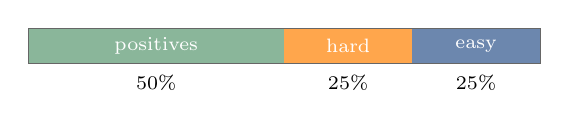
\begin{tikzpicture}[x=0.065cm,y=0.45cm]
        \fill[veripetgreen!70] (0,0) rectangle (50,1);
        \fill[orange!70] (50,0) rectangle (75,1);
        \fill[veripetblue!70] (75,0) rectangle (100,1);
        \draw[black!60] (0,0) rectangle (100,1);
        \node[white] at (25,0.5) {\scriptsize positives};
        \node[white] at (62.5,0.5) {\scriptsize hard};
        \node[white] at (87.5,0.5) {\scriptsize easy};
        \node[below] at (25,-0.05) {\scriptsize 50\%};
        \node[below] at (62.5,-0.05) {\scriptsize 25\%};
        \node[below] at (87.5,-0.05) {\scriptsize 25\%};
      \end{tikzpicture}
    \end{column}
  \end{columns}
\end{frame}

\begin{frame}{Verification: Prediction Examples}
  \centering
  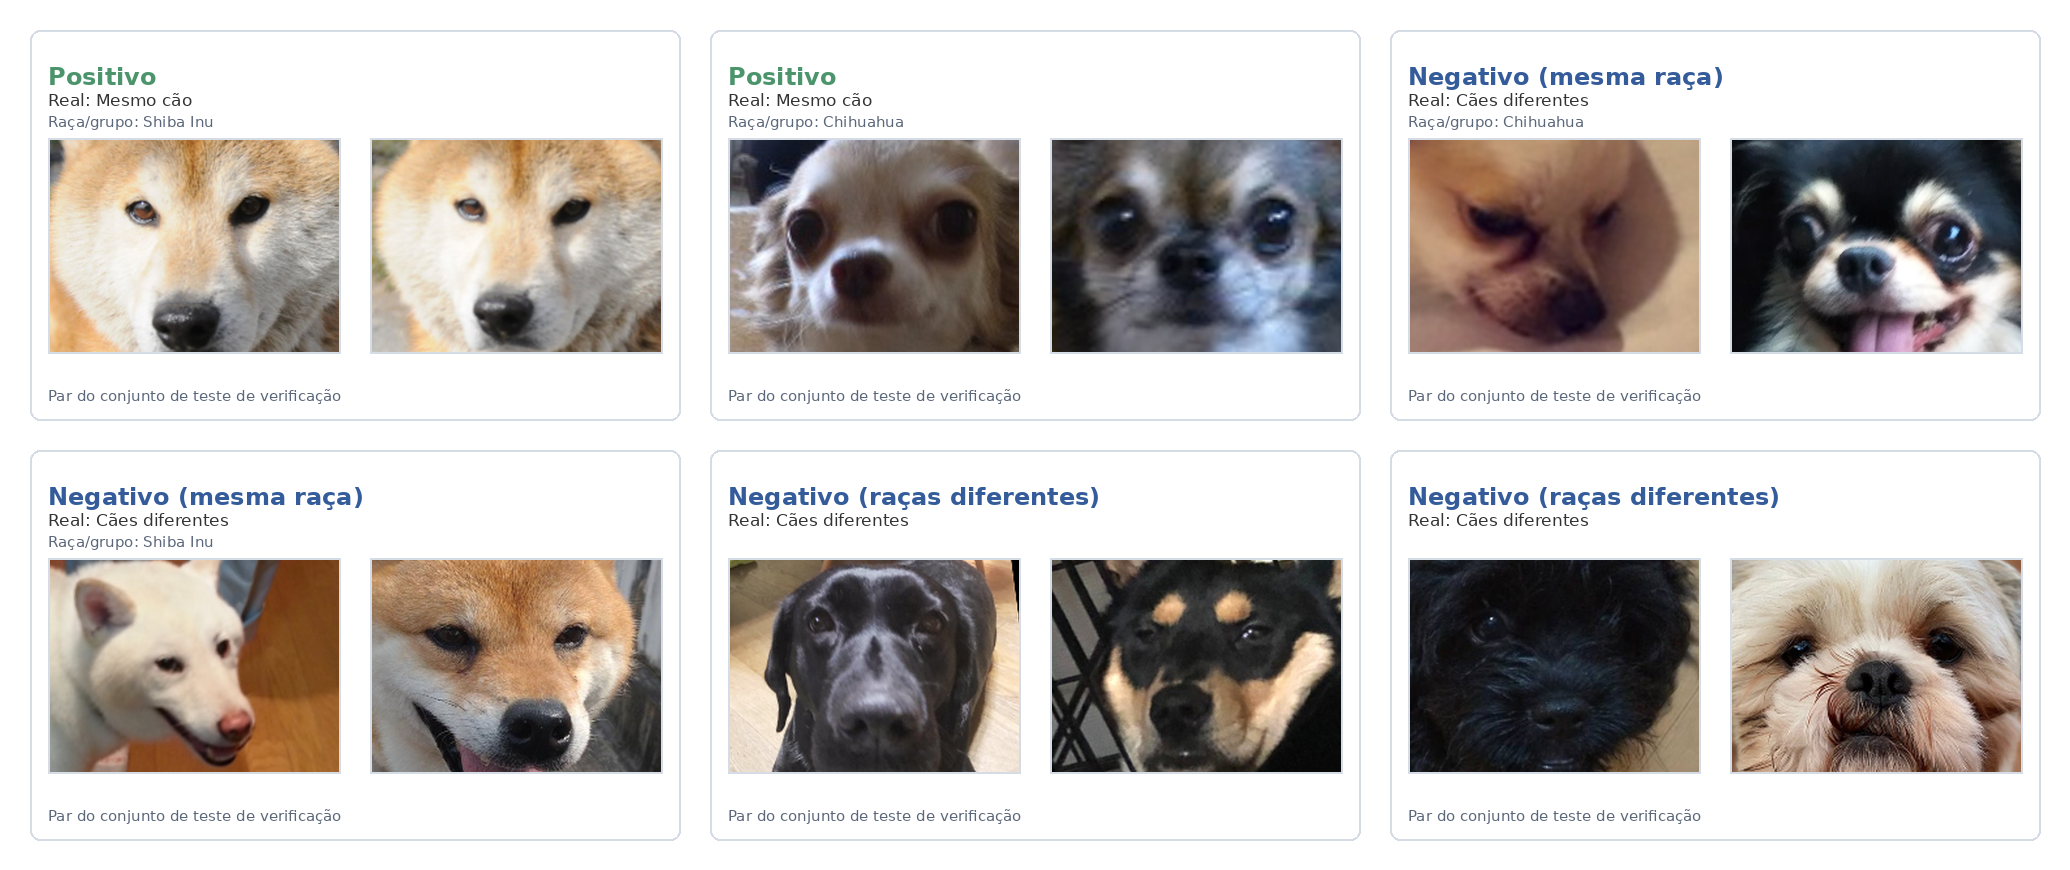
\includegraphics[width=0.98\textwidth,height=0.70\textheight,keepaspectratio]{prediction_examples_results.png}
\end{frame}

\begin{frame}{Verification: Softmax vs. ArcFace}
  \begin{center}
    \small Softmax and ArcFace are loss functions used to train identity embeddings.
  \end{center}
  \vspace{0.18cm}

  \begin{columns}[T,onlytextwidth]
    \begin{column}{0.52\textwidth}
      \begin{table}
        \centering
        \small
        \begin{tabular}{lrrr}
          \toprule
          Loss & AUC & Acc. & Intra-breed \\
          \midrule
          Softmax & 95.49\% & 86.31\% & 80.81\% \\
          ArcFace & 97.40\% & 92.52\% & 87.88\% \\
          \bottomrule
        \end{tabular}
      \end{table}
    \end{column}
    \begin{column}{0.43\textwidth}
      \begin{block}{ArcFace Gain}
        +6.21 percentage points in global accuracy and +7.07 percentage points in intra-breed accuracy.
      \end{block}
    \end{column}
  \end{columns}

  \vspace{0.35cm}
  \begin{center}
    \begin{minipage}{0.78\textwidth}
      \begin{alertblock}{Interpretation}
        Angular-margin learning forces clearer identity separation in the embedding space.
      \end{alertblock}
    \end{minipage}
  \end{center}
\end{frame}

\begin{frame}{Verification Curves and Score Distributions}
  \centering
  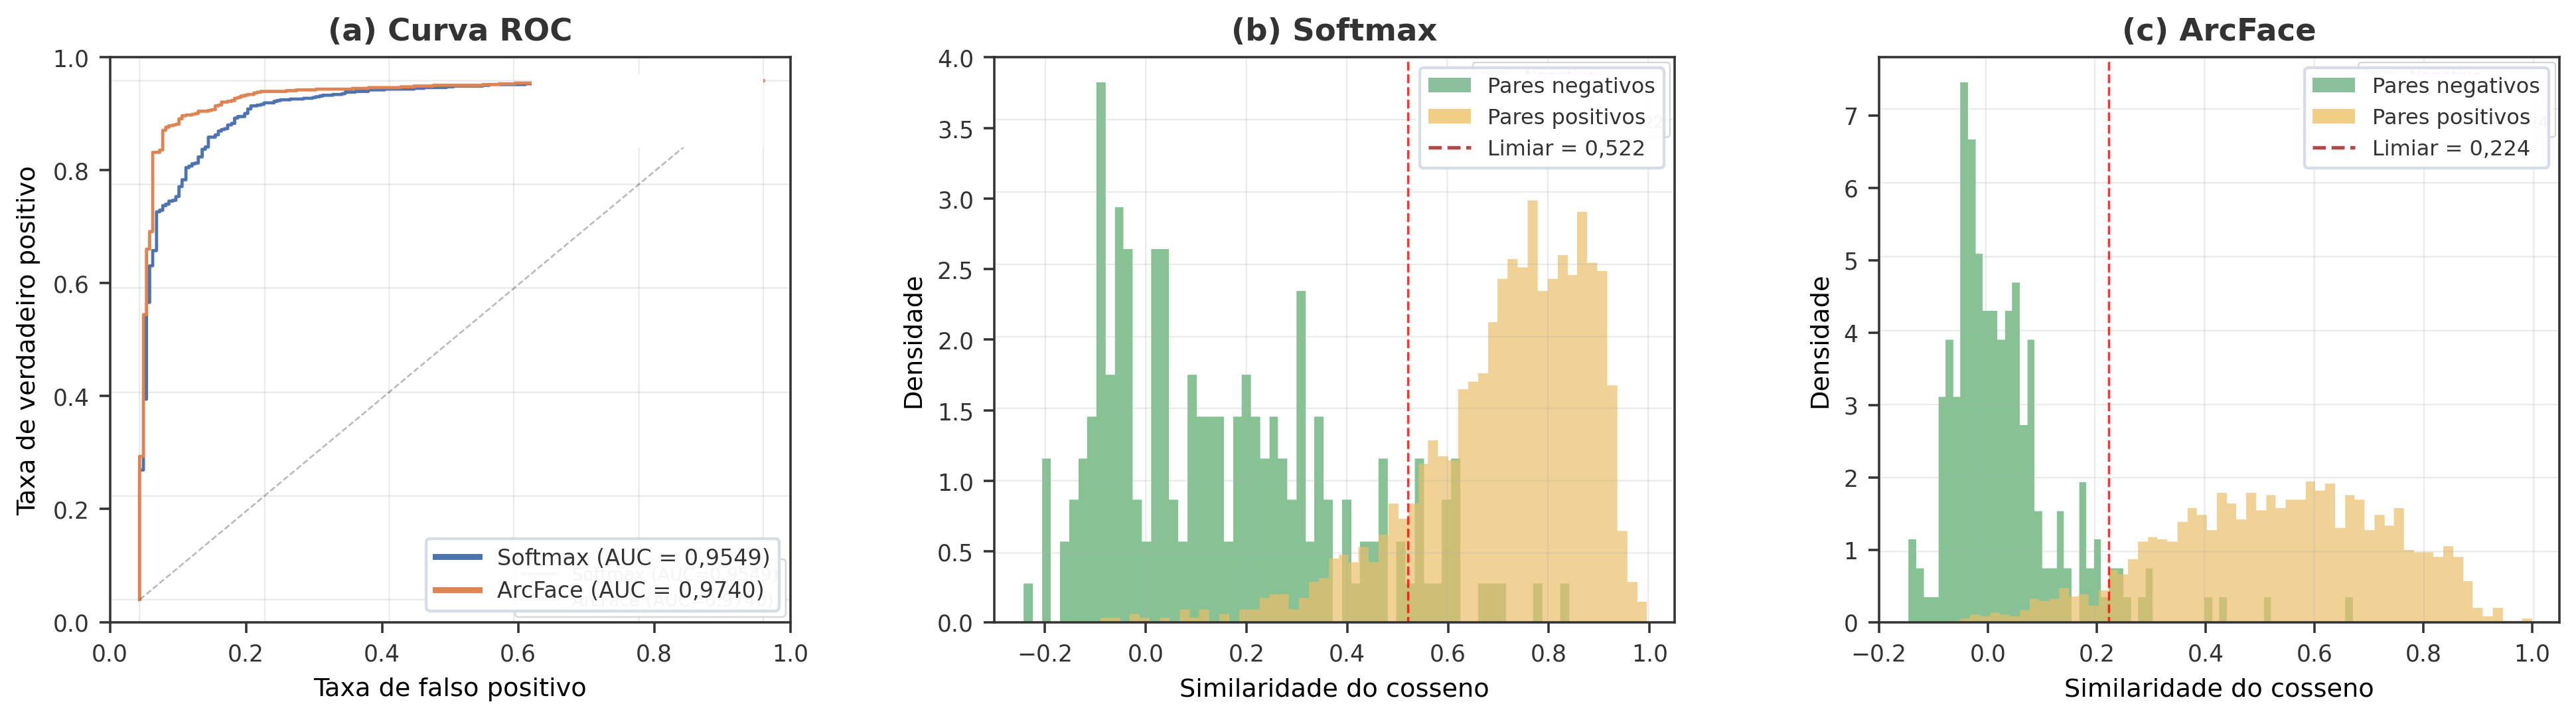
\includegraphics[width=0.96\textwidth,height=0.68\textheight,keepaspectratio]{results_comparison.png}
\end{frame}

\begin{frame}{Breed-Based Fusion Protocol}
  \begin{block}{Combined Signals}
    \begin{itemize}
      \item Verifier similarity: $s_{\text{verif}}$.
      \item Breed overlap:
      \[
        s_{\text{breed}}=\sum_{c=1}^{120}p_c(I_1)p_c(I_2)
      \]
      \item A pair can be rejected when breed compatibility is too low.
    \end{itemize}
  \end{block}

  \begin{columns}[T,onlytextwidth]
    \begin{column}{0.48\textwidth}
      \begin{alertblock}{Purpose}
        Test whether breed is a useful complementary signal for false-positive rejection.
      \end{alertblock}
    \end{column}
    \begin{column}{0.48\textwidth}
      \begin{block}{Comparison}
        Fusion and breed-only baselines are compared with the ArcFace verifier.
      \end{block}
    \end{column}
  \end{columns}
\end{frame}

\begin{frame}{Breed Classifier as Verification Filter}
  \begin{block}{Hypothesis}
    If two images receive incompatible breed predictions, this information could help reject false positives.
  \end{block}

  \begin{table}
    \centering
    \small
    \begin{tabular}{lrrrr}
      \toprule
      Method & Overall & Positives & Hard neg. & Easy neg. \\
      \midrule
      ArcFace verifier & 93.33\% & 92.80\% & 88.23\% & 99.49\% \\
      Breed Top-1 & 76.23\% & 56.34\% & 92.40\% & 99.83\% \\
      Breed overlap & 93.10\% & 92.22\% & 88.37\% & 99.59\% \\
      \bottomrule
    \end{tabular}
  \end{table}
\end{frame}

\begin{frame}{Discussion}
  \begin{columns}[T,onlytextwidth]
    \begin{column}{0.48\textwidth}
      \begin{block}{What Worked}
        \begin{itemize}
          \item ConvNeXt-Tiny reached 92.55\% accuracy across 120 breeds.
          \item ArcFace reached 97.40\% AUC for verification.
          \item Intra-breed analysis made evaluation more realistic.
        \end{itemize}
      \end{block}
    \end{column}
    \begin{column}{0.48\textwidth}
      \begin{block}{Observed Limits}
        \begin{itemize}
          \item Breed errors concentrate in visually close classes.
          \item PetFace has few images per identity and breed imbalance.
          \item Breed fusion did not produce a robust gain.
        \end{itemize}
      \end{block}
    \end{column}
  \end{columns}
\end{frame}

\begin{frame}{Scientific Impact}
  \begin{itemize}
    \item VeriPet separates category recognition from biometric identity verification.
    \item The results show that breed information is useful context, not a substitute for identity embeddings.
    \item ArcFace-style metric learning is a strong baseline for canine biometrics.
    \item Reporting intra-breed performance is essential for realistic animal-identification evaluation.
  \end{itemize}
\end{frame}

\begin{frame}{Reproducibility}
  \begin{block}{Repository}
    \texttt{https://github.com/mdrapha/veripet.git}
  \end{block}
  \begin{columns}[T,onlytextwidth]
    \begin{column}{0.48\textwidth}
      \begin{block}{Code}
        \begin{itemize}
          \item \texttt{src/veripet/research}
          \item Dataset contracts, models, losses, metrics, evaluation, plots.
        \end{itemize}
      \end{block}
    \end{column}
    \begin{column}{0.48\textwidth}
      \begin{block}{Workflows}
        \begin{itemize}
          \item \texttt{notebooks/colab}
          \item Classification, verification, thresholds, fusion, error analysis.
        \end{itemize}
      \end{block}
    \end{column}
  \end{columns}
\end{frame}

\begin{frame}{Conclusion}
  \begin{block}{Main Finding}
    Deep learning is viable for individual dog verification, especially when embeddings are trained with ArcFace.
  \end{block}
  \begin{itemize}
    \item Breed classification achieved high performance but remains difficult for visually similar breeds.
    \item Individual verification is the central biometric component.
    \item Breed information helps interpretation but should not be used as a strong replacement for verification.
    \item VeriPet provides a reproducible experimental baseline for canine biometrics.
  \end{itemize}
\end{frame}

\begin{frame}{Questions}
  \begin{center}
    
\includegraphics[height=1.2cm]{logo-unifesp.pdf}

    \vspace{1.2cm}
    {\Huge Thank you}

    \vspace{0.7cm}
    {\Large Questions?}
  \end{center}
\end{frame}

\appendix
\section*{Backup}

\begin{frame}{Backup}
  \begin{center}
    {\Huge Backup}

    \vspace{0.6cm}
    {\Large Supporting slides}
  \end{center}
\end{frame}

\begin{frame}{Breed Classification: Training}
  \centering
  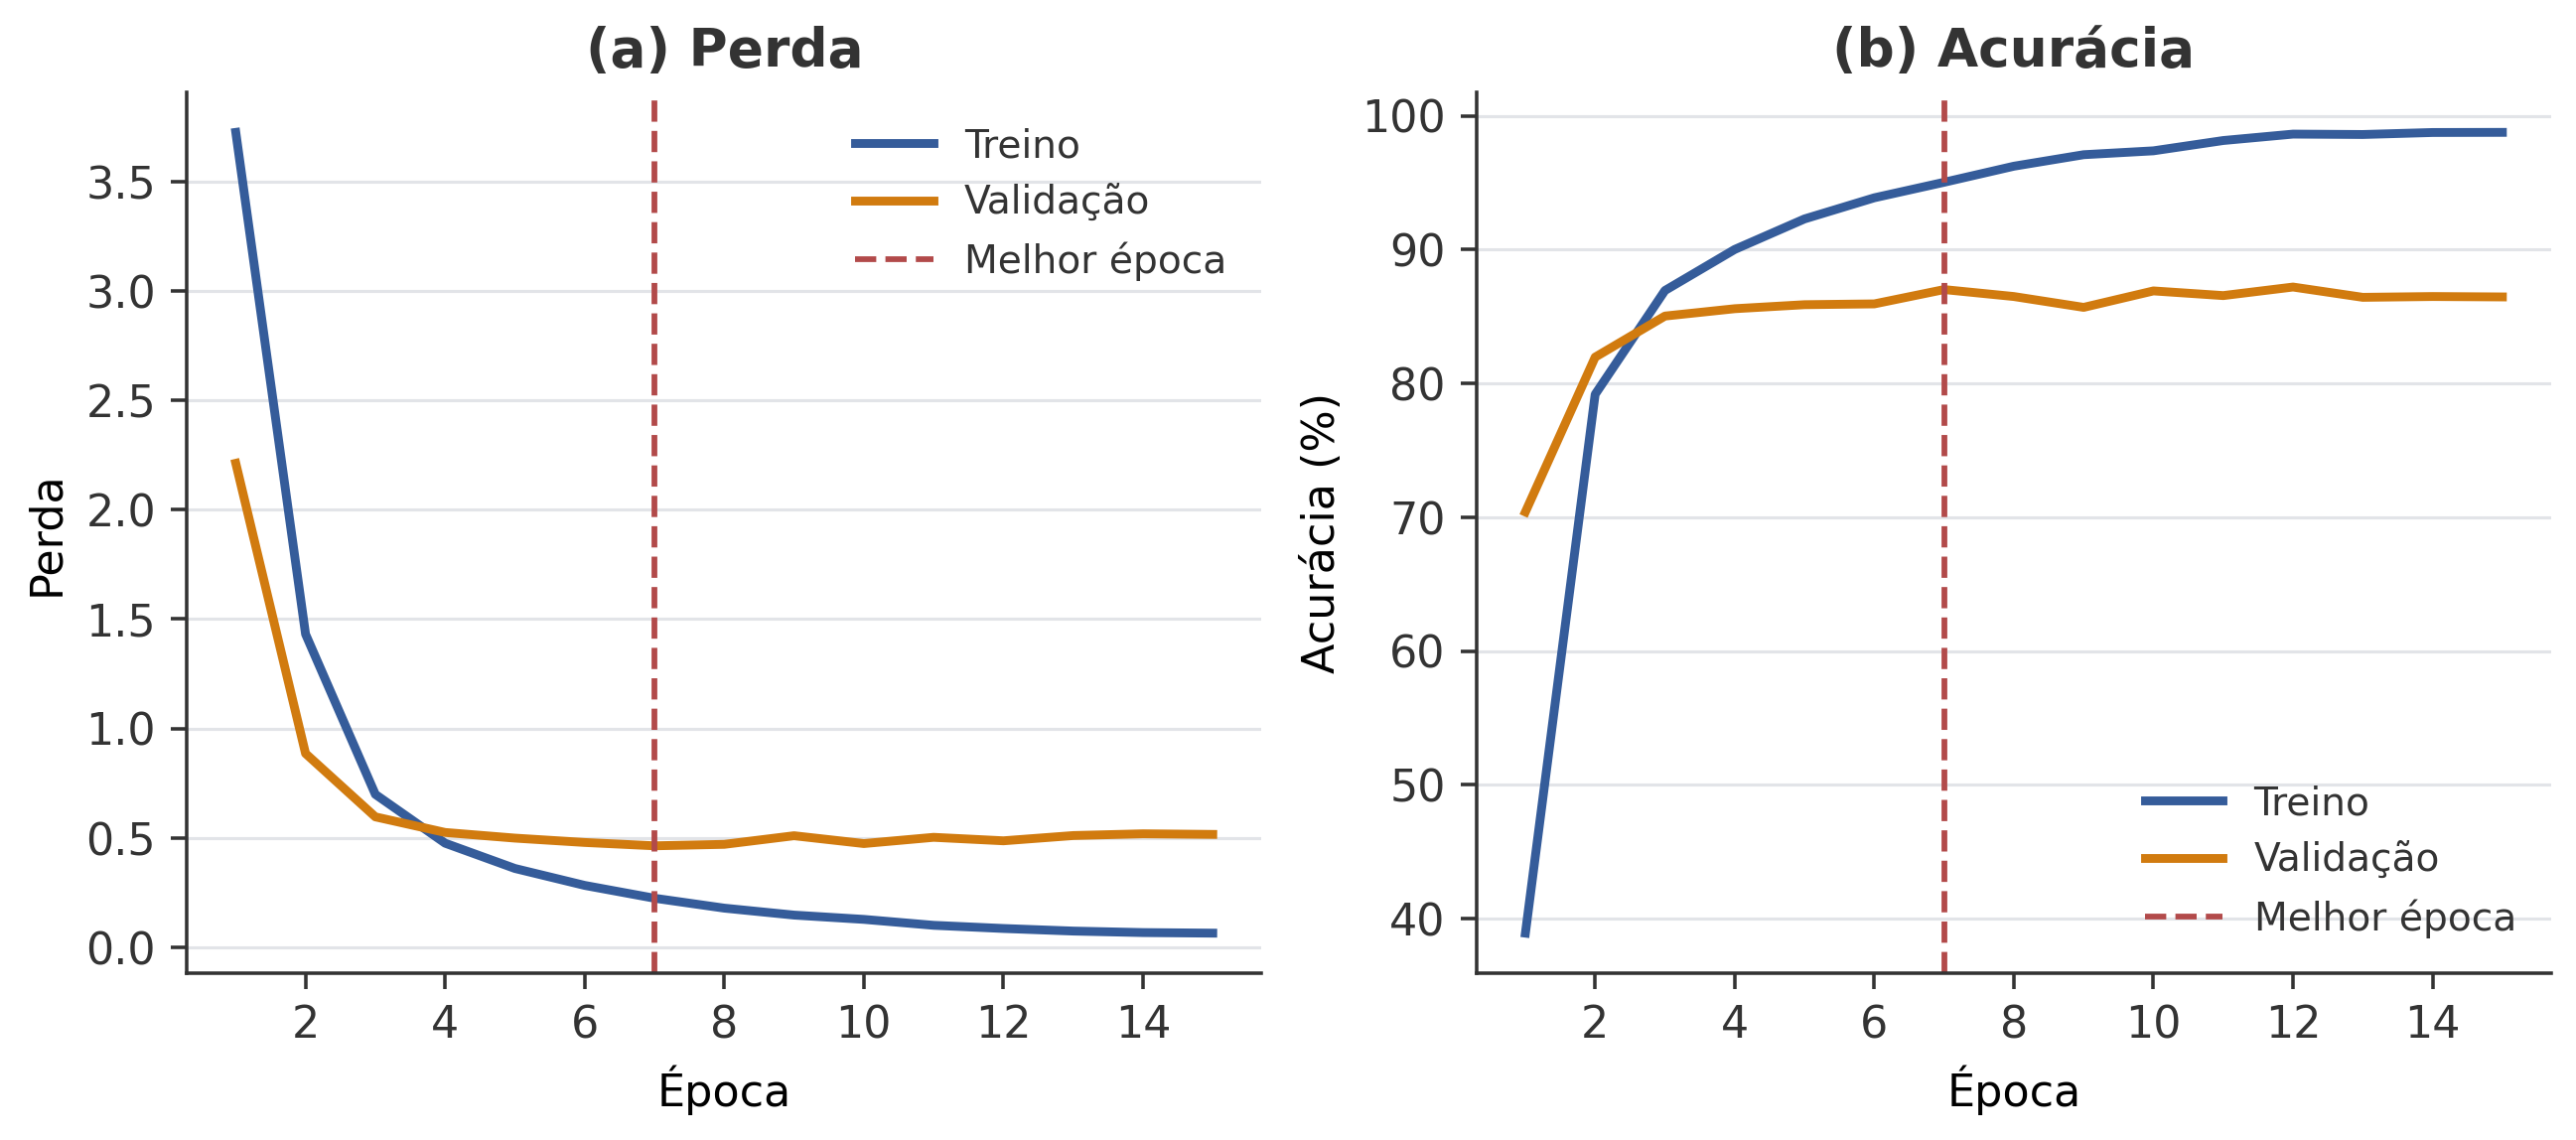
\includegraphics[width=0.92\textwidth,height=0.66\textheight,keepaspectratio]{curvas_treinamento.png}
\end{frame}

\begin{frame}{Verification: Training Curves}
  \centering
  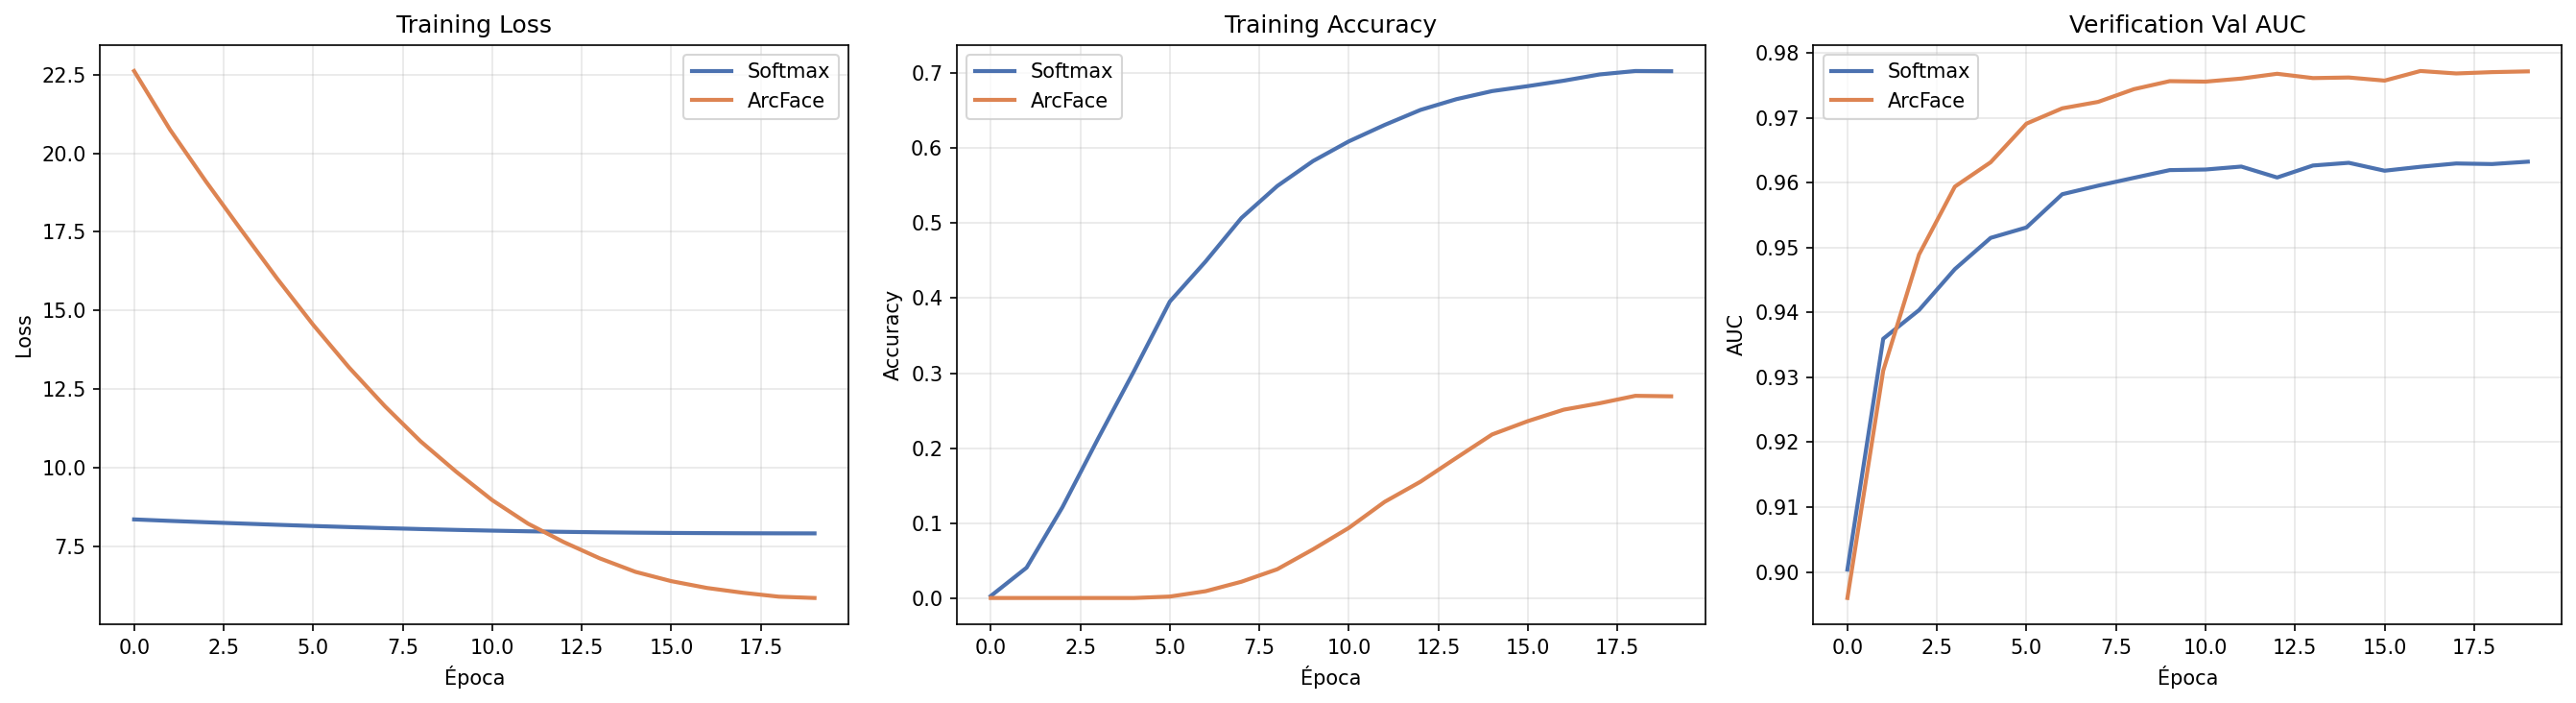
\includegraphics[width=0.94\textwidth,height=0.67\textheight,keepaspectratio]{training_curves.png}
\end{frame}

\end{document}
